\documentclass{article}
\usepackage[final]{neurips_2019}

% to avoid loading the natbib package, add option nonatbib:
%     \usepackage[nonatbib]{neurips_2019}

\usepackage[utf8]{inputenc} % allow utf-8 input
\usepackage[T1]{fontenc}    % use 8-bit T1 fonts
\usepackage{hyperref}       % hyperlinks
\usepackage{url}            % simple URL typesetting
\usepackage{booktabs}       % professional-quality tables
\usepackage{amsfonts}       % blackboard math symbols
\usepackage{nicefrac}       % compact symbols for 1/2, etc.
\usepackage{microtype}      % microtypography

\usepackage{amsmath}
\usepackage{graphicx}
\usepackage{float}
\usepackage[linesnumbered,ruled,vlined]{algorithm2e}
\usepackage{mdframed}
\usepackage[most]{tcolorbox}
\usepackage{subfig}
\usepackage{booktabs}
\renewcommand{\arraystretch}{1.2}  %make spacing of booktabs tables big

% Theorems
\usepackage{amsthm}
\renewcommand\qedsymbol{$\blacksquare$}
\makeatletter
\@ifclassloaded{article}{
    \newtheorem{definition}{Definition}[section]
    \newtheorem{example}{Example}[section]
    \newtheorem{theorem}{Theorem}[section]
    \newtheorem{corollary}{Corollary}[theorem]
    \newtheorem{lemma}{Lemma}[theorem]
}{
}
\makeatother

% Random Stuff
\setlength\unitlength{1mm}

\newcommand{\insertfig}[3]{
\begin{figure}[htbp]
\begin{center}
{\includegraphics[width=0.8 \textwidth]{#1}}
\end{center}
\caption{#2}\label{#3}
\end{figure}}

\newcommand{\insertxfig}[4]{
\begin{figure}[htbp]
\begin{center}
\leavevmode \centerline{\resizebox{#4\textwidth}{!}{\input
#1.pstex_t}}
\caption{#2} \label{#3}
\end{center}
\end{figure}}

\long\def\comment#1{}

\newcommand\norm[1]{\left\lVert#1\right\rVert}
\newcommand\abs[1]{\left\lvert#1\right\rvert}
\DeclareMathOperator*{\argmin}{arg\,min}
\DeclareMathOperator*{\argmax}{arg\,max}

% bb font symbols
\newfont{\bbb}{msbm10 scaled 700}
\newcommand{\CCC}{\mbox{\bbb C}}

\newfont{\bbf}{msbm10 scaled 1100}
\newcommand{\CC}{\mbox{\bbf C}}
\newcommand{\PP}{\mbox{\bbf P}}
\newcommand{\RR}{\mbox{\bbf R}}
\newcommand{\QQ}{\mbox{\bbf Q}}
\newcommand{\ZZ}{\mbox{\bbf Z}}
\renewcommand{\SS}{\mbox{\bbf S}}
\newcommand{\FF}{\mbox{\bbf F}}
\newcommand{\GG}{\mbox{\bbf G}}
\newcommand{\EE}{\mbox{\bbf E}}
\newcommand{\NN}{\mbox{\bbf N}}
\newcommand{\KK}{\mbox{\bbf K}}
\newcommand{\KL}{\mbox{\bbf KL}}
\newcommand{\MM}{\mbox{\bbf M}}

% Vectors
\renewcommand{\aa}{{\bf a}}
\newcommand{\bb}{{\bf b}}
\newcommand{\cc}{{\bf c}}
\newcommand{\dd}{{\bf d}}
\newcommand{\ee}{{\bf e}}
\newcommand{\ff}{{\bf f}}
\renewcommand{\gg}{{\bf g}}
\newcommand{\hh}{{\bf h}}
\newcommand{\ii}{{\bf i}}
\newcommand{\jj}{{\bf j}}
\newcommand{\kk}{{\bf k}}
\renewcommand{\ll}{{\bf l}}
\newcommand{\mm}{{\bf m}}
\newcommand{\nn}{{\bf n}}
\newcommand{\oo}{{\bf o}}
\newcommand{\pp}{{\bf p}}
\newcommand{\qq}{{\bf q}}
\newcommand{\rr}{{\bf r}}
\renewcommand{\ss}{{\bf s}}
\renewcommand{\tt}{{\bf t}}
\newcommand{\uu}{{\bf u}}
\newcommand{\ww}{{\bf w}}
\newcommand{\vv}{{\bf v}}
\newcommand{\xx}{{\bf x}}
\newcommand{\yy}{{\bf y}}
\newcommand{\zz}{{\bf z}}
\newcommand{\0}{{\bf 0}}
\newcommand{\1}{{\bf 1}}

% Matrices
\newcommand{\Ab}{{\bf A}}
\newcommand{\Bb}{{\bf B}}
\newcommand{\Cb}{{\bf C}}
\newcommand{\Db}{{\bf D}}
\newcommand{\Eb}{{\bf E}}
\newcommand{\Fb}{{\bf F}}
\newcommand{\Gb}{{\bf G}}
\newcommand{\Hb}{{\bf H}}
\newcommand{\Ib}{{\bf I}}
\newcommand{\Jb}{{\bf J}}
\newcommand{\Kb}{{\bf K}}
\newcommand{\Lb}{{\bf L}}
\newcommand{\Mb}{{\bf M}}
\newcommand{\Nb}{{\bf N}}
\newcommand{\Ob}{{\bf O}}
\newcommand{\Pb}{{\bf P}}
\newcommand{\Qb}{{\bf Q}}
\newcommand{\Rb}{{\bf R}}
\newcommand{\Sb}{{\bf S}}
\newcommand{\Tb}{{\bf T}}
\newcommand{\Ub}{{\bf U}}
\newcommand{\Wb}{{\bf W}}
\newcommand{\Vb}{{\bf V}}
\newcommand{\Xb}{{\bf X}}
\newcommand{\Yb}{{\bf Y}}
\newcommand{\Zb}{{\bf Z}}

% Calligraphic
\newcommand{\Ac}{{\cal A}}
\newcommand{\Bc}{{\cal B}}
\newcommand{\Cc}{{\cal C}}
\newcommand{\Dc}{{\cal D}}
\newcommand{\Ec}{{\cal E}}
\newcommand{\Fc}{{\cal F}}
\newcommand{\Gc}{{\cal G}}
\newcommand{\Hc}{{\cal H}}
\newcommand{\Ic}{{\cal I}}
\newcommand{\Jc}{{\cal J}}
\newcommand{\Kc}{{\cal K}}
\newcommand{\Lc}{{\cal L}}
\newcommand{\Mc}{{\cal M}}
\newcommand{\Nc}{{\cal N}}
\newcommand{\Oc}{{\cal O}}
\newcommand{\Pc}{{\cal P}}
\newcommand{\Qc}{{\cal Q}}
\newcommand{\Rc}{{\cal R}}
\newcommand{\Sc}{{\cal S}}
\newcommand{\Tc}{{\cal T}}
\newcommand{\Uc}{{\cal U}}
\newcommand{\Wc}{{\cal W}}
\newcommand{\Vc}{{\cal V}}
\newcommand{\Xc}{{\cal X}}
\newcommand{\Yc}{{\cal Y}}
\newcommand{\Zc}{{\cal Z}}

% Bold greek letters
\newcommand{\alphab}{\hbox{\boldmath$\alpha$}}
\newcommand{\betab}{\hbox{\boldmath$\beta$}}
\newcommand{\gammab}{\hbox{\boldmath$\gamma$}}
\newcommand{\deltab}{\hbox{\boldmath$\delta$}}
\newcommand{\etab}{\hbox{\boldmath$\eta$}}
\newcommand{\lambdab}{\hbox{\boldmath$\lambda$}}
\newcommand{\epsilonb}{\hbox{\boldmath$\epsilon$}}
\newcommand{\nub}{\hbox{\boldmath$\nu$}}
\newcommand{\mub}{\hbox{\boldmath$\mu$}}
\newcommand{\zetab}{\hbox{\boldmath$\zeta$}}
\newcommand{\phib}{\hbox{\boldmath$\phi$}}
\newcommand{\psib}{\hbox{\boldmath$\psi$}}
\newcommand{\thetab}{\hbox{\boldmath$\theta$}}
\newcommand{\taub}{\hbox{\boldmath$\tau$}}
\newcommand{\omegab}{\hbox{\boldmath$\omega$}}
\newcommand{\xib}{\hbox{\boldmath$\xi$}}
\newcommand{\sigmab}{\hbox{\boldmath$\sigma$}}
\newcommand{\pib}{\hbox{\boldmath$\pi$}}
\newcommand{\rhob}{\hbox{\boldmath$\rho$}}

\newcommand{\Gammab}{\hbox{\boldmath$\Gamma$}}
\newcommand{\Lambdab}{\hbox{\boldmath$\Lambda$}}
\newcommand{\Deltab}{\hbox{\boldmath$\Delta$}}
\newcommand{\Sigmab}{\hbox{\boldmath$\Sigma$}}
\newcommand{\Phib}{\hbox{\boldmath$\Phi$}}
\newcommand{\Pib}{\hbox{\boldmath$\Pi$}}
\newcommand{\Psib}{\hbox{\boldmath$\Psi$}}
\newcommand{\Thetab}{\hbox{\boldmath$\Theta$}}
\newcommand{\Omegab}{\hbox{\boldmath$\Omega$}}
\newcommand{\Xib}{\hbox{\boldmath$\Xi$}}

% mixed symbols
\newcommand{\sinc}{{\hbox{sinc}}}
\newcommand{\diag}{{\hbox{diag}}}
\renewcommand{\det}{{\hbox{det}}}
\newcommand{\trace}{{\hbox{tr}}}
\newcommand{\tr}{\trace}
\newcommand{\sign}{{\hbox{sign}}}
\renewcommand{\arg}{{\hbox{arg}}}
\newcommand{\var}{{\hbox{var}}}
\newcommand{\cov}{{\hbox{cov}}}
\renewcommand{\Re}{{\rm Re}}
\renewcommand{\Im}{{\rm Im}}
\newcommand{\eqdef}{\stackrel{\Delta}{=}}
\newcommand{\defines}{{\,\,\stackrel{\scriptscriptstyle \bigtriangleup}{=}\,\,}}
\newcommand{\<}{\left\langle}
\renewcommand{\>}{\right\rangle}
\newcommand{\Psf}{{\sf P}}
\newcommand{\T}{\top}
\newcommand{\m}[1]{\begin{bmatrix} #1 \end{bmatrix}}


\usepackage[final]{pdfpages}
\usepackage[shortlabels]{enumitem}

\title{Differential Geometry Final Project}
\author{%
 Tim Player \\
  Harvey Mudd College\\
  Claremont, CA 91711 \\
  \texttt{tplayer@hmc.edu} \\
}

\begin{document}
\maketitle

\begin{abstract}
    An algorithm for recovering the complete pose of a rocket from inertial data and outward-facing cameras was developed. Complete algorithms are presented for recovering the horizon from outward-facing videos, and for fusing the video pitch and yaw information with inertial sensors via an extended Kalman filter operating on orientation deviation states. With the filter data, the rocket achieved an apogee of $2,742$ meters and a top speed of  $324$ meters per second.
\end{abstract}

\section{Motivation}
Precisely localizing moving platforms using inertial sensors is a fundamental problem in robotics. These sensors, such as gyroscopes, accelerometers, and magnetometers, allow changes in position and orientation (together, ``pose") to be determined over short time scales in a process called \textit{dead reckoning}. This approach is used, for instance, in aerospace where precise estimates of aircraft pose may lead to safer landings. However, the cheapest sensors provide noisy measurements which cause dead-reckoning to be generally ineffective over long periods of time. 

MEMS magnetometers, which are used as digital compasses to provide estimates of orientation with respect to the Earth's magnetic field, can provide erroneous estimates due to the presence of magnetic material near the sensor, unmodeled geological perturbations in the Earth's field, miscalibration, and white observation noise. This can lead to uncertainty in orientation measurements on the order of several degrees \cite{introtoiner}. The error, in turn, causes exponentially-growing errors in position estimation, as we will discuss in Section \ref{sec:posest}. As a result, absolute measurements of orientation which are independent of magnetometers have direct utility in robotic state estimation.

This project implements direct orientation measurement via computer vision horizon estimation. Using inertial and visual data collected on a supersonic sounding rocket in April 2019, we develop an algorithm for pose estimation which incorporates visual horizon estimation as an independent, redundant measure of orientation to address the deficiencies of magnetometers. As shown in Fig. \ref{fig:horizon_overview}, cameras mounted inside of the rocket face opposite directions so they can see the horizon. As a result, changes in rocket attitude manifest in the camera image as coupled and opposite tilting, raising, or lowering of the horizon in each image. This allows direct estimation of pitch and yaw in a global frame.

In this paper, we first provide an explicit overview of the pose-estimation problem in section \ref{sec:posest} and detail some existing algorithms. In section \ref{sec:dynmod}, we develop the dynamical model used to represent the physical constraints of the rocket trajectory, including the parametrization of orientation with unit quaternions. Appendix \ref{sec:data} presents in more depth the available data collected during the April flights and the steps needed to prepare it for use in a sensor fusion algorithm. Section \ref{sec:algorithm} gives an overview of the multiplicative Extended Kalman Filter we use, and results follow.

%%%%%%%%%%%%%%%%%%%%%%%%%%%%   FIGURE  %%%%%%%%%%%%%%%%%%
\begin{figure}[ht]%
 \centering
 \subfloat[]{\includegraphics[width=5cm]{rocket_fov2.jpg}\label{fig:a}}\\
 \subfloat[]{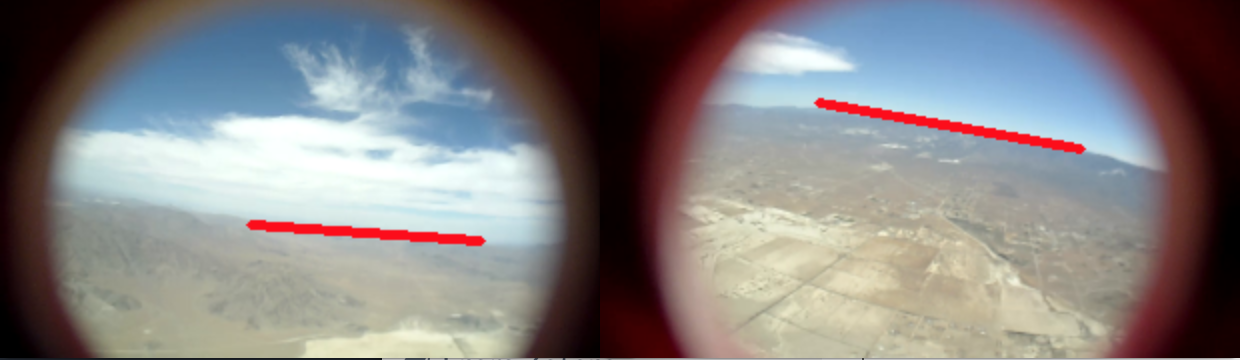
\includegraphics[width=5cm]{horiz.png}\label{fig:b}}%
 \caption{Visual horizon identification scheme during rocket flight. Approximate field of view of opposite-facing cameras is shown in red in sub-figure (a). Camera output is shown in sub-figure (b).}%
 \label{fig:horizon_overview}%
\end{figure}
%%%%%%%%%%%%%%%%%%%%%%%%%%%%%%%%%%%%%%%%%%%%%%%%%%%%%%%%%

\section{Pose Estimation Problem} \label{sec:posest}
The problem of \textit{sensor fusion} comprises strategies to intelligently combine observations from the various sensors which indirectly measure different elements of the platform's pose. Whereas the system's pose includes
\[
\{\text{\textit{x}-position,\textit{y}-position, \textit{z}-position, pitch, roll, yaw}\}
= \{x, y, z, r, p, y\},
\]
direct measurements of these items are not available. The gyroscope, for instance, observes the time-derivatives $\{\dot{r}, \dot{p}, \dot{y}\}$, and the accelerometer measures \textit{specific force}, which provides gravity-biased measurements of $\{\ddot{x}, \ddot{y}, \ddot{z} \}$ in a local frame. As discussed above, magnetometers provide a noisy absolute measurement of the orientation $\{r, p, y\}$. 

It is necessary to define several frames of reference. First, the \textit{body} frame $\textbf{b}$ is the coordinate frame of the moving rocket. This has the pitch axis $x_b$, yaw axis $y_b$, and roll axis $z_b$ shown in Fig. \ref{fig:axes}. 

The navigation frame $\textbf{n}$ is the coordinate frame in which we wish to localize the rocket, whose origin is at the launch pad. To this we ascribe the East, North, Up (ENU) triad. Note that both systems described have positive orientation. 

To be fully comprehensive, we must also include the \textit{inertial} frame \textbf{i} and the \textit{Earth} frame \textbf{e}. The accelerometer and rate gyroscope take measurements with respect to the inertial frame rather than the navigation frame or body frame, and thus the effects of Coriolis acceleration caused by the Earth's rotation and body acceleration caused by the Earth's orbit may be factored in. However, as the rocket flight is on the order of minutes, the frames do not become significantly different so we make the valid simplifying assumption that the navigation frame \textbf{n} is inertial, and we remove \textbf{i} and \textbf{e} from further discussion.

%%%%%%%%%%%%%%%%%%%%%%%%%%%%   FIGURE  %%%%%%%%%%%%%%%%%%
\begin{figure}[htbp]%
    \centering
      	\framebox{
            \subfloat{
                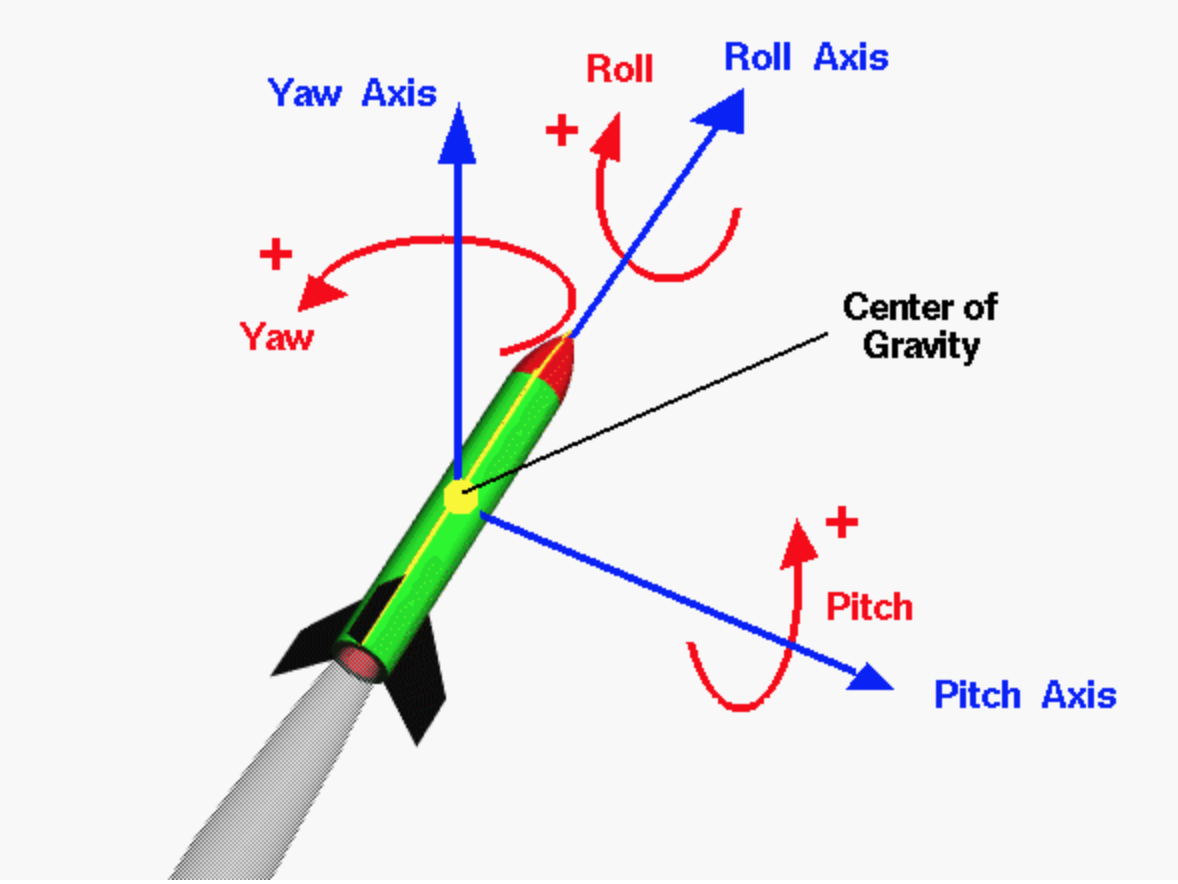
\includegraphics[width=8cm]{rotations.png} 
            }
        }
    \caption{Attitude axis conventions. Camera 1's aperture lies on the pitch axis.}%
    \label{fig:axes}
\end{figure}
%%%%%%%%%%%%%%%%%%%%%%%%%%%%%%%%%%%%%%%%%%%%%%%%%%%%%%%%%

To achieve a pose in the navigation frame based on measurements taken in the body frame, we must correct for the presence of gravity in the accelerometer measurements prior to integrating. As shown in Fig. \ref{fig:dr}, the rocket's orientation is first estimated via direct measurement with the magnetometer and by integrating of rate gyroscope values from the last time step. With this known orientation — a rotation between the \textbf{b} and \textbf{n} frames — the direction of gravity is known. Then gravity can be subtracted from the accelerometer readings to provide a measurement of true rocket acceleration in the navigation frame rather than specific force. Lastly, this acceleration is integrated twice to arrive at velocity and position.

\begin{figure}[ht]
  \centering
  \fbox{
  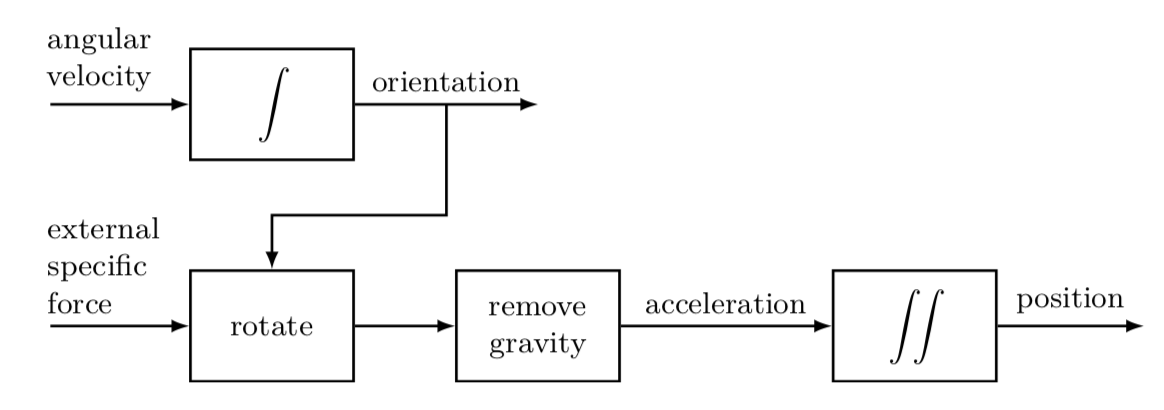
\includegraphics[width=0.7\textwidth]{dr.png}
    }
  \caption{Schematic illustration of dead-reckoning, where the accelerometer measurements (external specific force) and the gyroscope measurements (angular velocity) are integrated to position and orientation. From \cite{1}.}
  \label{fig:dr}
\end{figure}

To estimate pose, our approach to dead reckoning must intelligently utilize all data. Specifically, at each step $t$ along the rocket's trajectory we seek to quantify a conditional belief distribution regarding the rocket's pose $x_t$
\[ \label{eq:cond}
bel(t) = p(x_t | z_{1:t}),
\]
where $z_{1:t}$ are all of the measurements available from sensors through times $1$ through $t$. Under the Markov assumption, which is that our description of the rocket's state is complete enough that the knowledge of a prior state specifies belief of future states as well, then Eq. \ref{eq:cond} reduces to
\[
bel(t) = p(x_t | x_{t-1}, z_t),
\]
which is to say that the information from all measurements $z_{1:t-1}$ is included in the state $x_{t-1}$. This forms the basis of the Bayes Filter in general. We will implement a specific closed-form solution of the Bayes Filter in section \ref{sec:algorithm}.

\section{Quaternion Orientation Parametrization}
To model the orientation of the rocket, several parametrizations are available. The orientation of the rocket is given as a rotation from the navigation frame to the body frame of the rocket. Rotations are succinctly represented in matrix form as the set of all orthogonal linear transformations with unit determinant. That is, rotations form the special orthogonal group $SO(n)$. In three dimensions, 
\[
SO(3) = \left\{A \in M_{3\times 3} \,|\, A^TA = I, \qquad \det A = 1 \right\}.
\]

The set of all rotations $SO(3)$ is a group, so it has, for all $A \in SO(3)$, an inverse $A^{-1}$. Above, you can see that $A^{-1} = A^T$. Additionally, $SO(3)$ is closed under multiplication, the associative property applies, and the identity element $I \in SO(3)$. In fact, $SO(3)$ is a \textit{Lie group}, since it has manifold structure and an exponential map from the corresponding Lie algebra \cite{kok}.

Although the above matrix representation has an intuitive interpretation as the change-of-basis matrix representing the projection of each body-frame basis vector onto the navigation frame basis triad, it is inconvenient to work directly with matrices due to problems numerical instability and the high-dimensionality intrinsic to matrices. In fact, we choose to represent the orientation of the rocket as a \textit{unit quaternion}, an identical parametrization of $SO(3)$.

A unit quaternion $q$ is a member of the Hamiltonian numbers such that 
\[
q = (q_0 \, q_1 \, q_2 \, q_3)^\top = 
\begin{pmatrix}
q_0\\
q_v
\end{pmatrix}, 
\qquad q \in \RR^4, \qquad \norm{q} = 1.
\]

As Hamiltonian numbers, the three elements of $q_v$ behave similarly to the cross product in $\RR^3$, such that 
\[
i^2 = j^2 = k^2 = ijk = -1.
\]

Unit quaternions may be thought of as directly representing an rotation vector. That is, any orientation can be specified by indicating a unit axis of rotation $\eta^v = (x, y, z)^\top$ and an angle $\alpha$ to rotate a given basis triad about the axis. In fact,
\[
q^{uv}(\eta^v, \alpha) = 
\begin{pmatrix}
\cos \frac{\alpha}{2}\\
\sin \frac{\alpha}{2} \eta^v
\end{pmatrix}.
\]

A vector $u \in \RR^4$ can then be rotated using quaternion multiplication, defined such that 
\[
x^u = q^{uv} \odot x^v \odot (q^{uv})^C,
\]
where $(q^{uv})^C = q^{vu}$ denotes the quaternion complement, defined as
\[
q^C = (q_o (-q_v)^\top)^\top.
\]
As equivalent representations of the special orthogonal group, we may convert between unit quaternions and rotation matrices via their corresponding exponential maps from rotation vectors. In the remainder of this paper, we will use the mappings 
\begin{equation}
\label{eq:expq}
    q = \exp_q(\eta) = 
    \begin{pmatrix}
\cos \norm{\eta}_2\\
\sin \norm{\eta}_2 \frac{\eta}{\norm{\eta}_2}
\end{pmatrix}
\end{equation}
and
\begin{equation}
\label{eq:expr}
    R = \exp_R([\eta \times]) = I_3 + \sin (\norm{\eta}_2)\left[\frac{\eta}{\norm{\eta}_2} \times \right] + (1 - \cos(\norm{\eta}_2) \left[\frac{\eta}{\norm{\eta}_2} \times \right]^2
\end{equation}
where $[v \times]$ denotes the standard matrix cross product. This will allow us to make the approximations, for small $\eta$, that
\begin{equation}
\label{eq:expqapprox}
    \exp_q(\eta) \approx \begin{pmatrix}
    1\\
    \eta
    \end{pmatrix}
\end{equation}
\begin{equation}
\label{eq:exprapprox}
    \exp_R(\eta) \approx I_3 + [\eta \times].
\end{equation}



\section{Dynamic Model} \label{sec:dynmod}

We borrow the dynamics equations from \cite{introtoiner} to relate the position $p_t^n$, velocity $v_t^n$, and orientation to the measured acceleration and gyroscope inputs via
\begin{align}
\begin{pmatrix}
    p_{t + 1}^n\\
    v_{t + 1}^n\\
    q_{t + 1}^{nb}
    \end{pmatrix} &=
    \begin{pmatrix}
    p_t^n + T v_t^n + \frac{T^2}{2}(R_t^{nb}  y_{a,t} + g^n + e_{p,a,t})\\
    v_t^n + T (R_t^{nb}  y_{a,t} + g^n + e_{v,a,t})\\
    q_{t}^{nb} \odot \exp_q\left(\frac{T}{2} (y_(\omega, t-1) - e_{\omega,t})\right)
    \end{pmatrix}
\end{align}
where 
\begin{align*}
    e_{p,a,t} &\sim \mathcal{N}(0, \Sigma_a), 
    &e_{v,a,t} &\sim \mathcal{N}(0, \Sigma_a),\\
    e_{\omega,t} &\sim \mathcal{N}(0, \Sigma_\omega).
\end{align*}

with $\Sigma_a = \sigma_a^2 I_3$ and $\Sigma_2 = \sigma_w^2 I_3$. Then, the problem becomes to estimate the state using known time series data $y_{a_t}$ and $y_{\omega,t}$ for each step $t$.

Additionally, measurements of orientation are available from the magnetometer as
\begin{equation}
    y_{m,t} = R_t^{bn} m^n + e_{m,t}.
\end{equation}


\subsection{Measurement Equations for Camera Pitch and Yaw}
\label{sec:pitchyawmeas}
%%%%%%%%%%%%%%%%%%%%%%%%%%%%   FIGURE  %%%%%%%%%%%%%%%%%%
\begin{figure}[htbp]%
    \centering
      	\framebox{
            \subfloat{
                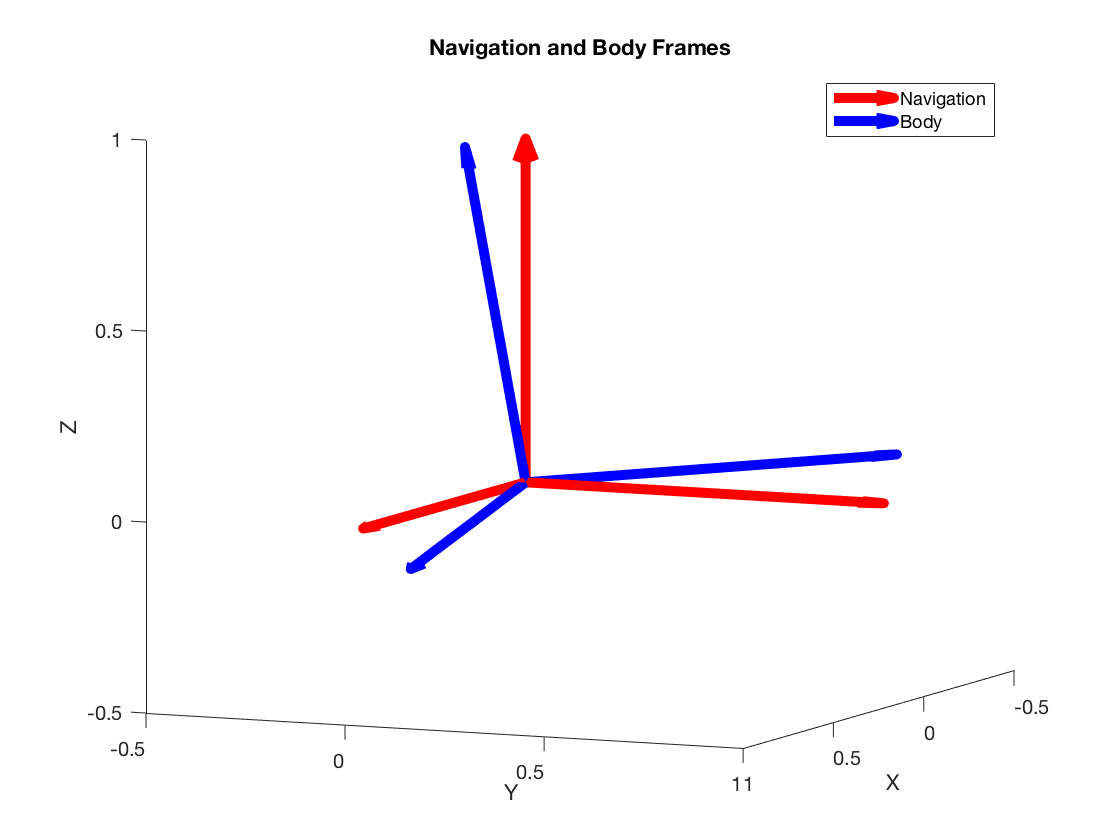
\includegraphics[width=8cm]{frames.png} 
            }
        }
    \caption{Navigation and body frames representing a rotation matrix $R_{nb}$.}%
    \label{fig:frames}
\end{figure}
%%%%%%%%%%%%%%%%%%%%%%%%%%%%%%%%%%%%%%%%%%%%%%%%%%%%%%%%%

A thorough treatment of the image formation process involves concepts from projective geometry and optics; such a treatment is not given here. Instead we direct the reader to Appendix \ref{sec:image_posest} or Szeliski's \textit{Computer Vision: Algorithms and Applications}. For our purposes, we only intend to recover the pitch and yaw of the rocket from the two camera horizons available. This does not require significant projective geometry, though the following intuitive relationship is derived from it.

Figures \ref{fig:horizon_overview} and \ref{fig:axes} are useful in determining this relationship. Since Camera 1 is directed along the pitch axis of the rocket and Camera 2 is directed in the opposite direction, the rotation and height of the horizon in the image directly describe the global pitch and yaw of the rocket respectively.

Furthermore, consider the body-frame axes shown in blue in Figure \ref{fig:frames}. The rotation matrix 
\[
R^{nb} = [v_1 \, v_2 \, v_3]
\]
is comprised of the three columns representing the local yaw, pitch, and roll axes expressed in the global $x$, $y$, and $z$ basis. The rocket's pitch and yaw angles are therefore directly related to the projection of $v_1$ and $v_2$ onto the global $z$ axis. In fact, since the vectors of $R^{nb}$ are unit vectors, the pitch and yaw of the rocket are given by 
\begin{align}
    p_t &= \sin^{-1} [R_t^{nb}]_{3,2},\\
    y_t &= \sin^{-1} [R_t^{nb}]_{3,1},
\end{align}
where $R_t^{nb}$ is the rocket's rotation matrix at time $t$. 

This relationship is verified experimentally. Figure \ref{fig:attcompare} shows that the angular values calculated from video frames from Camera 1 and 2 closely track the predicted pitch and yaw values \textit{before} using the camera as an input to the sensor fusion scheme.

It is straightforward to determine $p_t$ and $y_t$ after identifying the horizon in the camera images through the technique given in Appendix \ref{sec:cvalg}. Figure \ref{fig:b} shows the view from the two cameras with horizon slopes $\theta_1$ and $\theta_2$ and heights $h_1$ and $h_2$. Then,
under a small angle approximation, the measurements of pitch and yaw become
\begin{align*}
    y_p &= \frac{\theta_2 - \theta_1}{2},\\
    y_y &= (0.0073) \, \frac{h_2 - h_1}{2} ,
\end{align*}
where the constant factor in the computation of $y_y$ relates the sensitivity of image pixels to perturbations about the yaw axis. Together, these measurements provide an independent measurement of rocket attitude relative to the magnetometer alone, which eliminates the degree of freedom originating from inability identify rocket rotation parallel to the magnetic field.

%%%%%%%%%%%%%%%%%%%%%%%%%%%%   FIGURE  %%%%%%%%%%%%%%%%%%
\begin{figure}[htbp]%
    \centering
      	\framebox{
            \subfloat{
                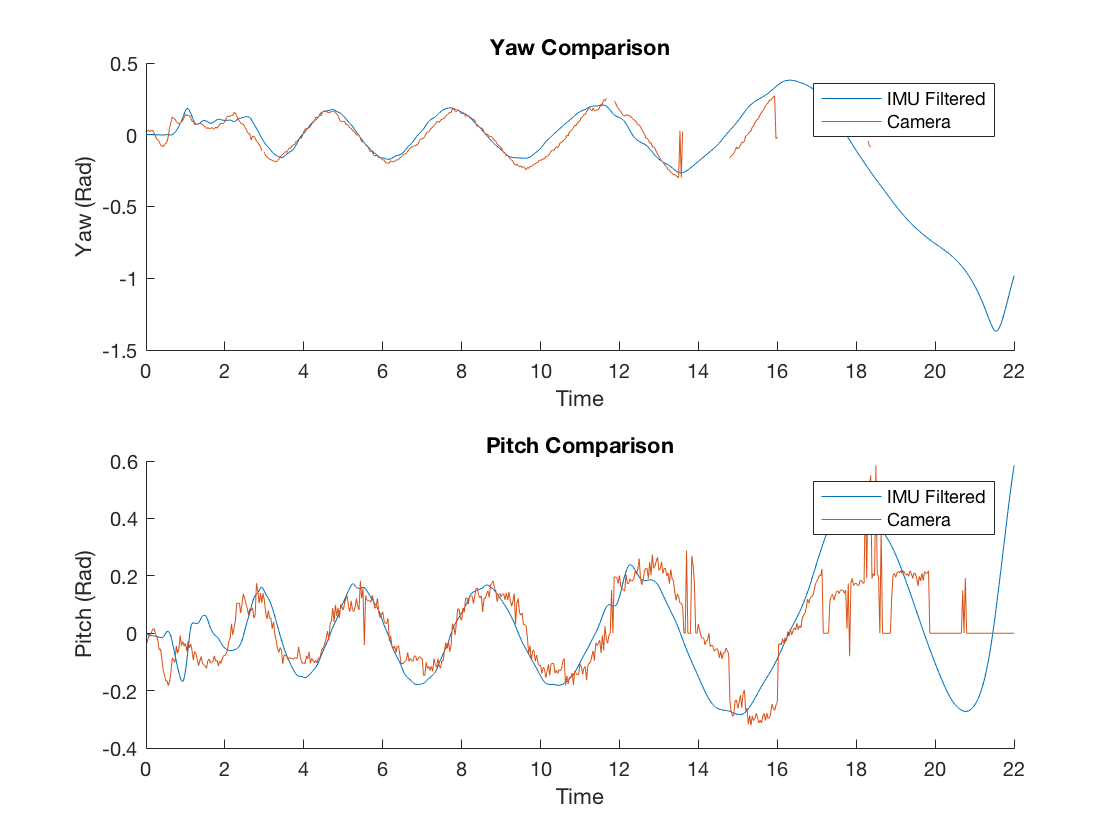
\includegraphics[width=8cm]{attitude_comparison.png} 
            }
        }
    \caption{Comparison of yaw and pitch values calculated from images with those calculated from inertial data. The granularity in the camera pitch is an artefact of the sensitivity of the Hough line-detecting transform to irregularities in the horizon.}%
    \label{fig:attcompare}
\end{figure}
%%%%%%%%%%%%%%%%%%%%%%%%%%%%%%%%%%%%%%%%%%%%%%%%%%%%%%%%%

\section{Sensor Fusion Algorithm} \label{sec:algorithm}
We will use the multiplicative Extended Kalman Filter with a quaternion orientation estimation, modified to achieve pose estimation rather than orientation alone. The unmodified algorithm is from \cite{introtoiner}.

This Extended Kalman Filter operates on \textit{orientation deviations} rather than orientations alone. Rather than keeping track of the four-element orientation quaternion, only the three-element incremental rotation vector is recorded. Due to Euler's theorem, this representation is sufficient to store the entire state history at a given time. 

As a consequence of working with orientation \textit{deviations}, the measurement matrix $H$ includes only the derivative of the measurement relationship. This will not be explained in detail in this draft, but its derived in \cite{introtoiner}.

Additionally, a complete derivation of the Kalman filter algorithm is given in \cite{appliedkalman}, and a fascinating visual derivation is available at \hyperlink{https://www.bzarg.com/p/how-a-kalman-filter-works-in-pictures/}{this link}. However, these results will not be reproduced here.

% derivation of effect of measurement derivative for pitch, yaw

\begin{algorithm}
\DontPrintSemicolon % Some LaTeX compilers require you to use \dontprintsemicolon instead
\KwIn{Inertial data $\{ y_{a,t}, y_{\omega,t}\}_{t=1}^N$, magnetometer data $\{y_{m,t}\}_{t=1}^N$ and covariance matrices $\Sigma_\omega$, $\Sigma_a$, and $\Sigma_m$.}
\KwOut{An estimate of the state $\{x, y, z, v_x, v_y, v_z, \eta_i, \eta_j, \eta_k\}$ and orientation $\tilde{q}_{t | t}^{nb}\,$  for $t = 1, ... , N$.}
Compute $\tilde{q}_{1 | 1}^{nb}\,$ using the TRIAD method and set the initial state covariance $P_{1|1}$.\\
\For{$t = 2, ..., N$} {
  \begin{enumerate}[(a)]
      \item Time Update
\begin{align}
    \hat{x}_{t | t -1} = 
    \begin{pmatrix}
    p_{t | t -1}^n\\
    v_{t | t -1}^n\\
    \hat{\eta}_{t | t -1}^n
    \end{pmatrix} &=
    \begin{pmatrix}
    p_t^n + T v_t^n + \frac{T^2}{2}(R_t^{nb}  y_{a,t} + g^n)\\
    v_t^n + T (R_t^{nb}  y_{a,t} + g^n)\\
    \mathbf{0}_{3\times1}
    \end{pmatrix},\\
    \tilde{q}_{t | t - 1}^{nb} &=  \tilde{q}_{t - 1 | t - 1}^{nb} \odot \exp_q\left(\frac{T}{2} y_(\omega, t-1) \right),\\
    P_{t | t-1} &= F_t P_{t | t-1} F_t^\top + G_{t-1} Q G_{t-1}^\top
\end{align}
with 
\begin{align*}
    G_{t-1} &= 
    \begin{pmatrix}
    T I_6 &\mathbf{0}\\
    \mathbf{0} &\tilde{R}_{t | t - 1}^{nb}
    \end{pmatrix},&
    Q &= \begin{pmatrix}
    I_6 &\mathbf{0}\\
    \mathbf{0} &\Sigma_\omega
    \end{pmatrix},& 
    F_t &= \begin{pmatrix}
    I_3 &T I_3 &-\frac{T^2}{2}(R_{t-1}^{nb}  [y_{a,t} \times] \\
    \mathbf{0} &I_3 & -T(R_{t-1}^{nb}  [y_{a,t} \times] \\
    \mathbf{0} &\mathbf{0}  &I_3
    \end{pmatrix}. 
\end{align*}
      \item Measurement Update
      \begin{align}
          \hat{\eta}_t^n &= K_t \left( y_t - \hat{y}_{t|t-1} \right),\\
          \tilde{P}_{t|t} &= P_{t | t-1} - K_t S_t K_t^\top,
      \end{align}
with
    \begin{align*}
        y_t &= \begin{pmatrix}
        y_{m,t} \\
        y_{p,t} \\
        y_{y,t}
        \end{pmatrix},&
        %
        \hat{y}_{t|t-1}  &= \begin{pmatrix}
        \tilde{R}_{t | t-1}^{bn}  m^n\\
        \sin^{-1} \left([\tilde{R}_{t | t-1}^{nb}]_{3,2}\right)\\
        \sin^{-1} \left([\tilde{R}_{t | t-1}^{nb}]_{3,1}\right)
        \end{pmatrix},\\
        S_t &= H_t P_{t | t-1} H_t^\top + R,&
        K_t &= P_{t | t-1} H_t S_{t}^{-1}\\
        H_t &= \begin{pmatrix}
        \mathbf{0} &\tilde{R}_{t | t-1}^{bn} [m^v \times]\\
        %
        \mathbf{0} & \frac{1}{\sqrt{1 - [\tilde{R}_{t | t-1}^{nb}]_{3,2}}} \left([\tilde{R}_{t | t-1}^{nb}]_{2,2}, \, \tilde{R}_{t | t-1}^{nb}]_{2,1},\, 0 \right)\\
        %
         \mathbf{0} & \frac{1}{\sqrt{1 - [\tilde{R}_{t | t-1}^{nb}]_{3,1}}} \left([\tilde{R}_{t | t-1}^{nb}]_{2,1},\, \tilde{R}_{t | t-1}^{nb}]_{1,1},\, 0 \right)\\
        \end{pmatrix}&
        R &= \begin{pmatrix}
        \Sigma_m &\mathbf{0} &\mathbf{0}\\
        \mathbf{0} & \Sigma_p &\mathbf{0}\\
        \mathbf{0} &\mathbf{0} & \Sigma_y 
        \end{pmatrix}
    \end{align*}
    \item Relinearize
    \begin{equation}
        \tilde{q}_{t | t}^{nb} = \exp_q \left( \frac{\hat{\eta}_t^n}{2}\right) \odot \tilde{q}_{t | t -1}^{nb}
    \end{equation}
  \end{enumerate}
}
\caption{Extended Kalman filter for pose estimation with orientation deviation state}
\label{algo:max}
\end{algorithm}

\section{Results}
The algorithm successfully predicted the trajectory of the rocket. Figure \ref{fig:trajectory} shows the Kalman-filtered prediction of the ascent trajectory. The orange circles show the GPS locations that were available during the descent, which carried the rocket to the East due to westerly wind. The GPS was unavailable while the rocket was rising because commercial GPS devices shut off if they are going very fast. The fact that the estimated rocket position is very close to the known GPS coordinate suggests the accuracy of this approach.

%%%%%%%%%%%%%%%%%%%%%%%%%%%%   FIGURE  %%%%%%%%%%%%%%%%%%
\begin{figure}[htbp]%
    \centering
      	\framebox{
            \subfloat{
                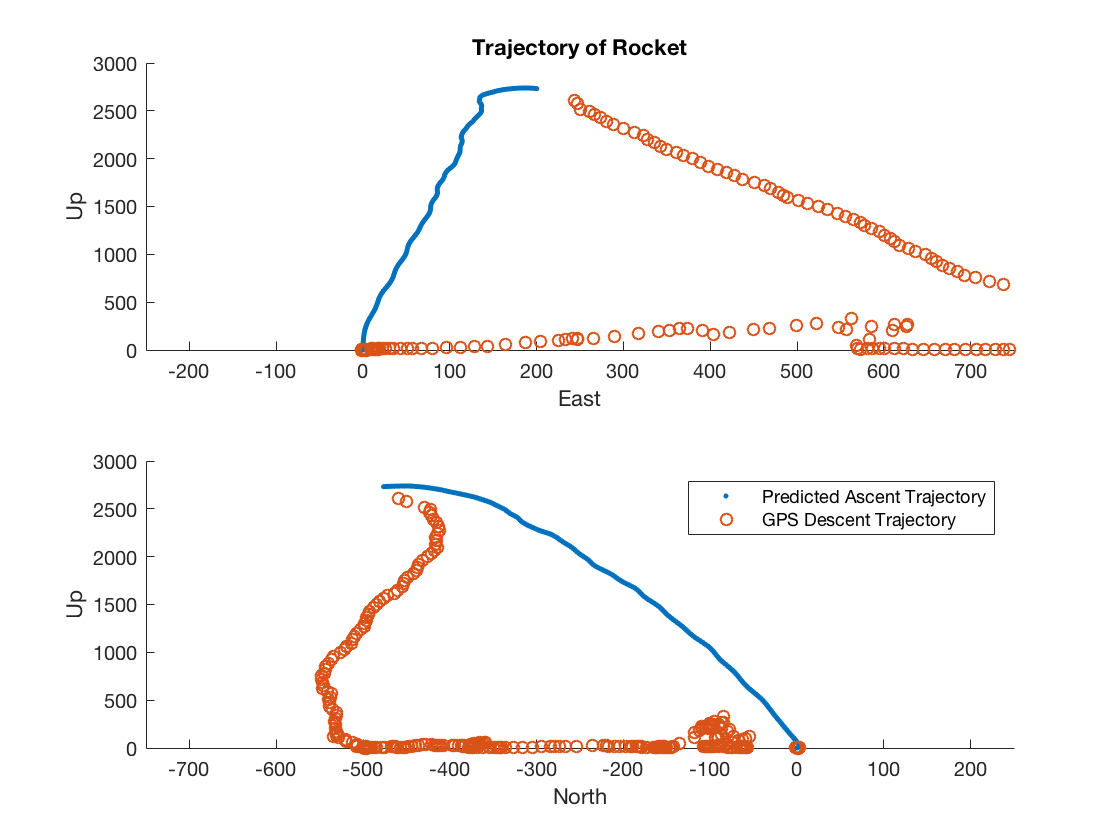
\includegraphics[width=10cm]{trajectory_2D.png} 
            }
        }
    \caption{Kalman-filtered trajectory of the rocket.}%
    \label{fig:trajectory}
\end{figure}
%%%%%%%%%%%%%%%%%%%%%%%%%%%%%%%%%%%%%%%%%%%%%%%%%%%%%%%%%

Figure \ref{fig:sphere} shows the traces of the local yaw, pitch, and roll axes during the first second of flight. This figure demonstrates the successful operation of the rate gyroscopes as well as the orientation-deviation update algorithm. Shown in black is the vector cross product
\[
y_\omega \times R^{nb},
\]
which projects the angular derivative of the system onto the tangent bundle of $So(2)$ in order to give a sense of the direction the system is evolving. In this case, the rocket is rotating clockwise around the roll axis.
%%%%%%%%%%%%%%%%%%%%%%%%%%%%   FIGURE  %%%%%%%%%%%%%%%%%%
\begin{figure}[htbp]%
    \centering
      	\framebox{
            \subfloat{
                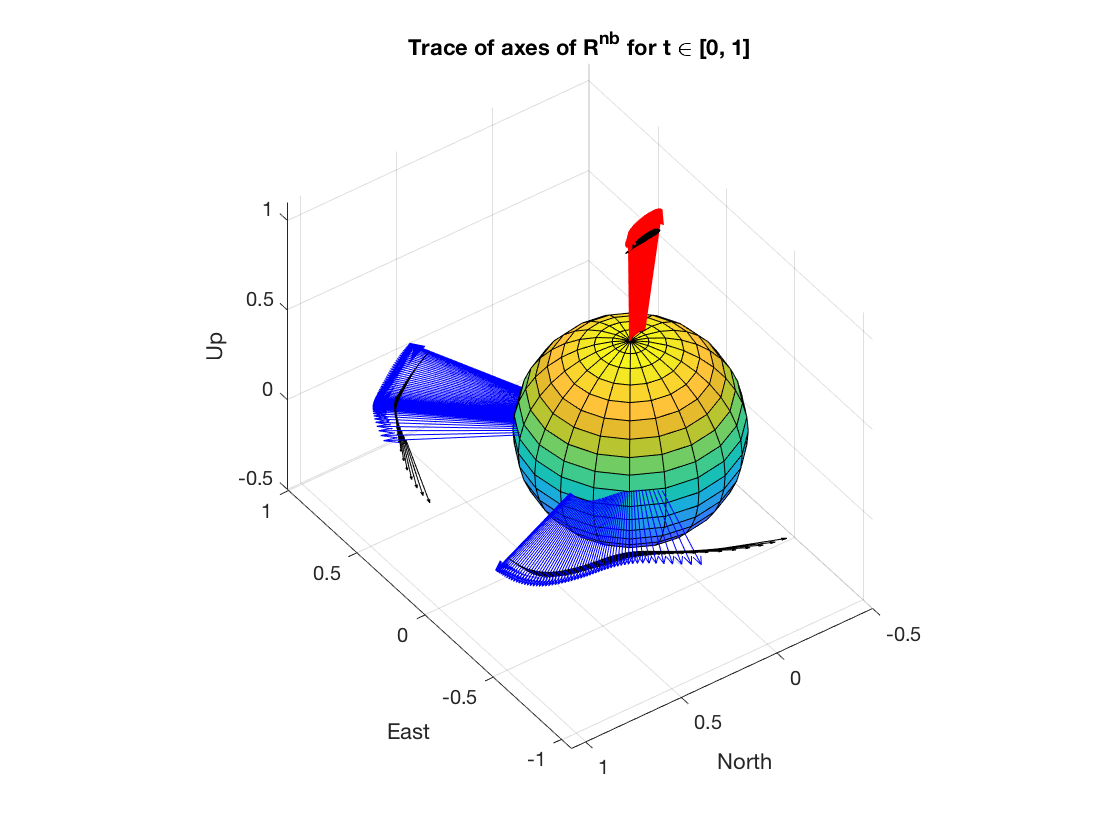
\includegraphics[width=10cm]{orientation_sphere.png} 
            }
        }
    \caption{Trace of the three columns of $R^nb$ during the first second of flight.}%
    \label{fig:sphere}
\end{figure}
%%%%%%%%%%%%%%%%%%%%%%%%%%%%%%%%%%%%%%%%%%%%%%%%%%%%%%%%%

Figure \ref{fig:unc_ellipses} shows the one-standard-deviation uncertainty ellipses at several points throughout the trajectory. The covariance was modified during the operation of the Kalman filter by the quadratic dynamics update and then the Kalman measurement update, as 
\begin{align*}
    P_{t | t-1} &= F_t P_{t | t-1} F_t^\top + G_{t-1} Q G_{t-1}^\top\\
    \tilde{P}_{t|t} &= P_{t | t-1} - K_t S_t K_t^\top.
\end{align*}
Because the system's position was not directly observable, the dynamics update dominated the behavior of the covariance matrix, resulting in approximately quadratic growth. Additionally, the model was highly sensitive to the initial uncertainty in the position estimate.

%%%%%%%%%%%%%%%%%%%%%%%%%%%%   FIGURE  %%%%%%%%%%%%%%%%%%
\begin{figure}[htbp]%
    \centering
      	\framebox{
            \subfloat{
                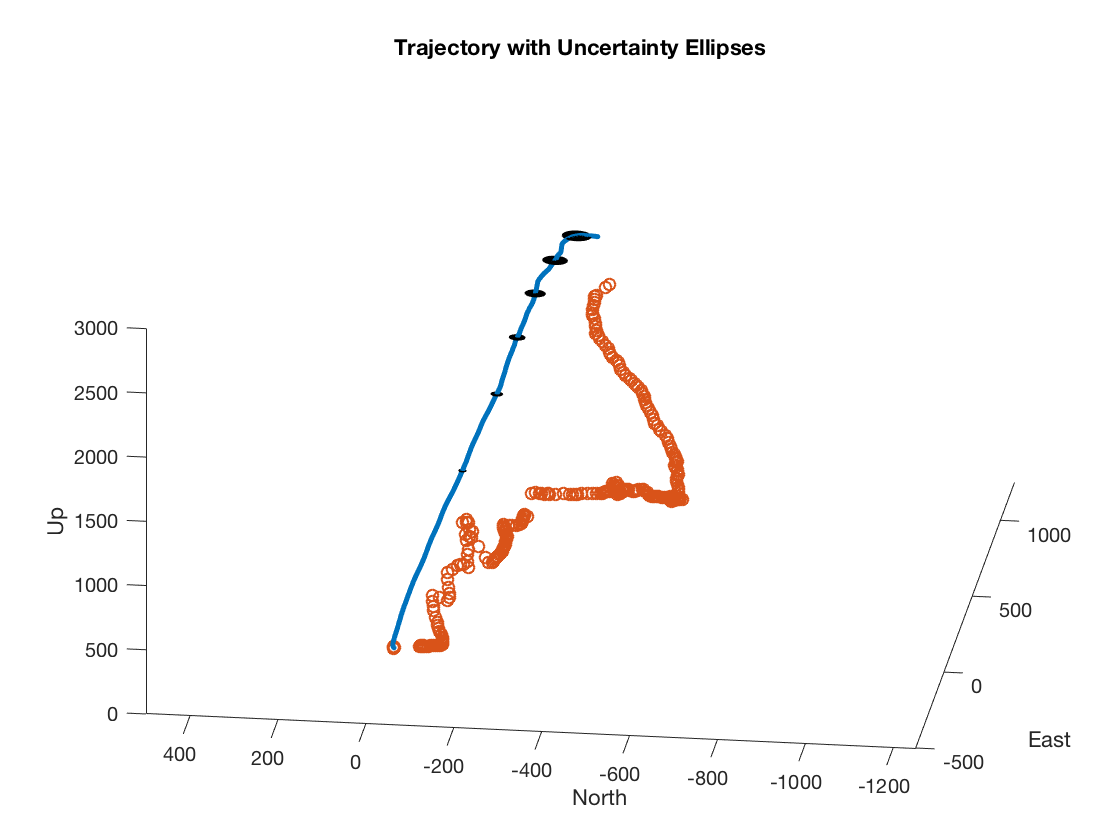
\includegraphics[width=10cm]{uncertainty_ellipses.png} 
            }
        }
    \caption{Trajectory including growing ellipses of uncertainty associated with positional covariance.}%
    \label{fig:unc_ellipses}
\end{figure}
%%%%%%%%%%%%%%%%%%%%%%%%%%%%%%%%%%%%%%%%%%%%%%%%%%%%%%%%%
% figure: quadratic growth in projected position error due to dynamics

\section{Conclusion}
The algorithm shown here achieved a reasonable estimate of the rocket's trajectory, while operating on the $SE(3)$ manifold. Understanding the derivation of these results has relied heavily on concepts from the study of differential geometry. 

Future fruitful work would continue draw on concepts from the study of differential geometry. Of particular interest are:
\begin{itemize}
    \item a lower dimensional parametrization of the system configuration
    \item an efficient method to integrate arbitrary distributions for measurement and state transition probabilities
    \item a computationally efficient approach to broader problem of inertial-visual simultaneous localization and mapping
\end{itemize}

\appendix
\newpage
\section{Data Handling} \label{sec:data}
Our data-processing pipeline must include the following.
\begin{enumerate}
    \item Find initial GPS location on the launch pad.
    \item Convert GPS data (not available during ascent) into meters from origin
    \item Apply laboratory bias-calibrations to raw accelerometer, gyroscope, and magnetometer data.
    \item Flip magnetometer $x$, $y$ aces to get right-handed system
    \item Scale magnetometer dimensions individually to normalize to $(-1, 1)$.
    \item Scale magnetometer readings so that at every step $t$ the $L_2$ norm is $1$.
    \item Get initial magnetometer orientation from the pre-launch sample mean. Also get sensor variance.
    \item Resample magnetometer using smooth interpolation.
    \item Convert gyroscope data to radians/sec.
    \item Convert accelerometer data to meters/sec using local gravitational constant.
    \item Get acceleration baseline from pre-launch sample mean. Also get sensor variance.
    \item Resample accelerometer and gyroscope data.
    \item \label{camerastep}Determine the global pitch and yaw corresponding to each image.
    \item Smooth the roll using complementary filter.
    \item Determine initial orientation using TRIAD method.
\end{enumerate}
This sequence of pre-processing steps should yield a unified set of relevant time-series data for sensor fusion. However, item \ref{camerastep} deserves more elaboration. We do so below. 

\subsection{Computer Vision Algorithm for Horizon Estimation}
\label{sec:cvalg}
An algorithm to automatically detect the horizon was implemented in OpenCV. The algorithm works by translating the image to an HSV (hue, saturation, and value) colorspace and identifying the sky. The edges of the sky region are then identified, and a straight line is fitted to the horizon. More specifically, the algorithm
\begin{enumerate}
    \item Makes a mask that includes the sky but not the ground, using an HSV tranform and thresholding.
    \item Finds the edges of that mask using Canny edge detection.
    \item Picks the longest edge. Assumes that contains the horizon.
    \item Crops the image to only examine the central rectangle (and not the edges of the circular window).
    \item Uses Hough line transform to identify a long straight line.
\end{enumerate}

An example set of computer vision intermediate steps is shown in Fig. \ref{fig:cv_alg}.

%%%%%%%%%%%%%%%%%%%%%%%%%%%%   FIGURE  %%%%%%%%%%%%%%%%%%
\begin{figure}[H]%
 \centering
 \subfloat[]{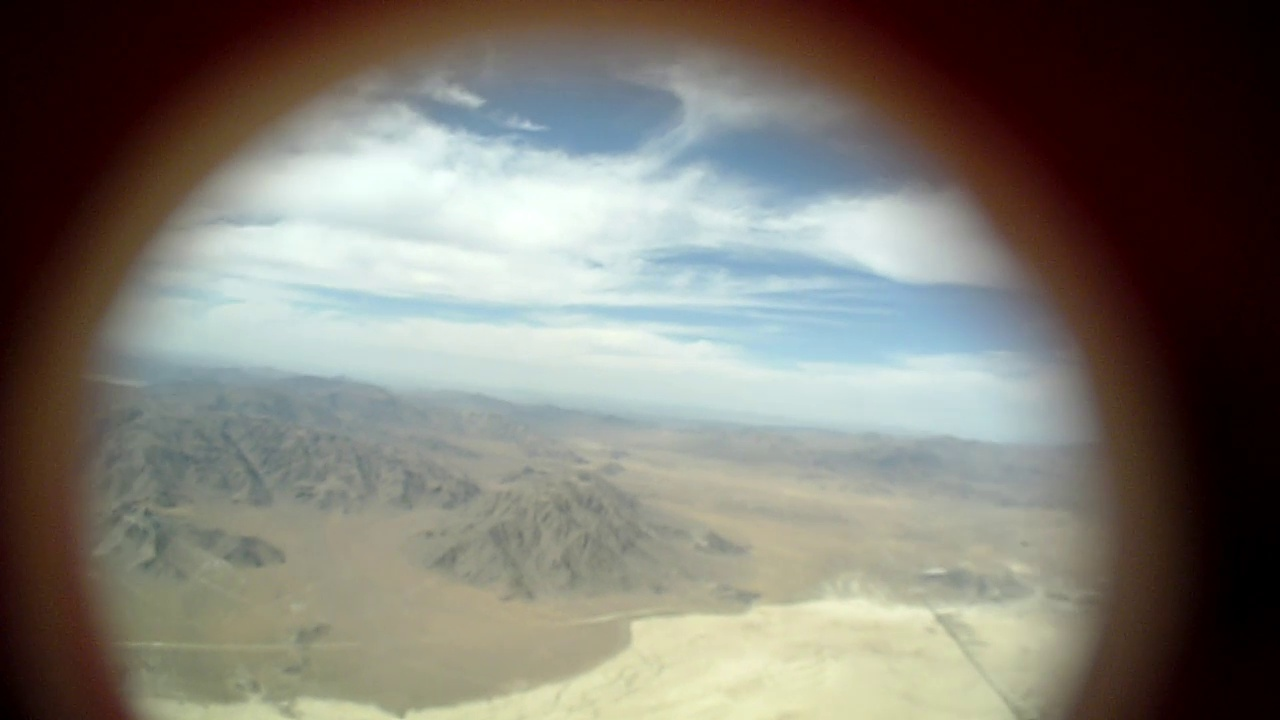
\includegraphics[width=3cm]{frame1_r.jpg}}\\
 \subfloat[]{
\includegraphics[width=3cm]{mask.png}}%
 \subfloat[]{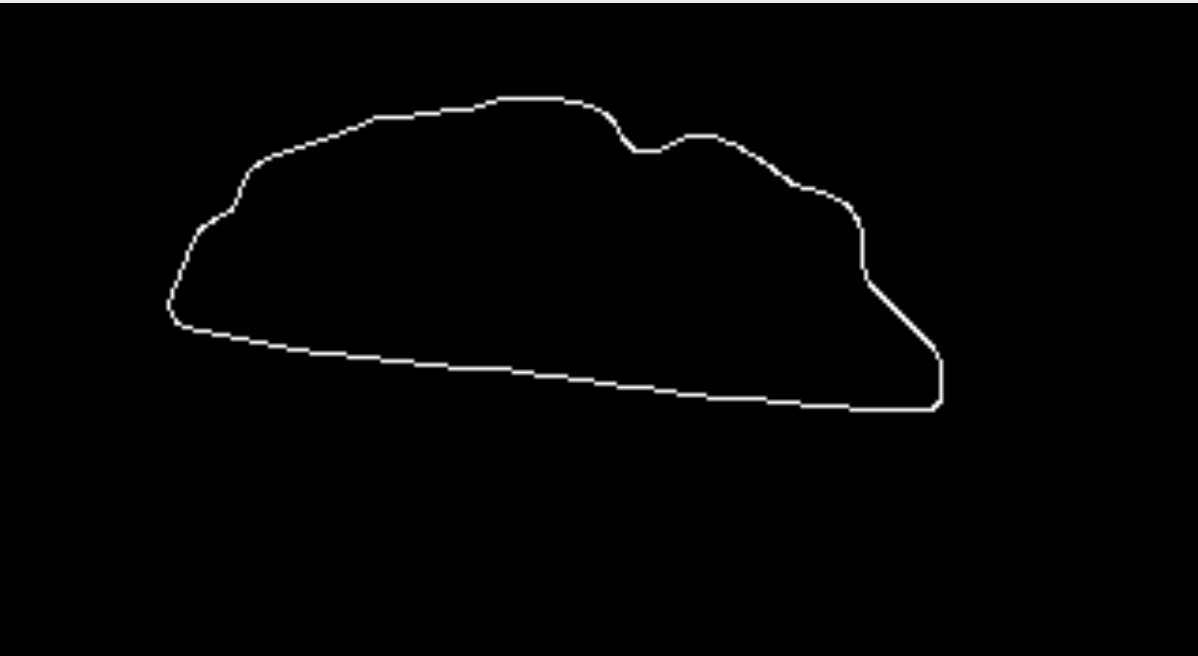
\includegraphics[width=3.1cm]{edges.png}}\\
 \subfloat[]{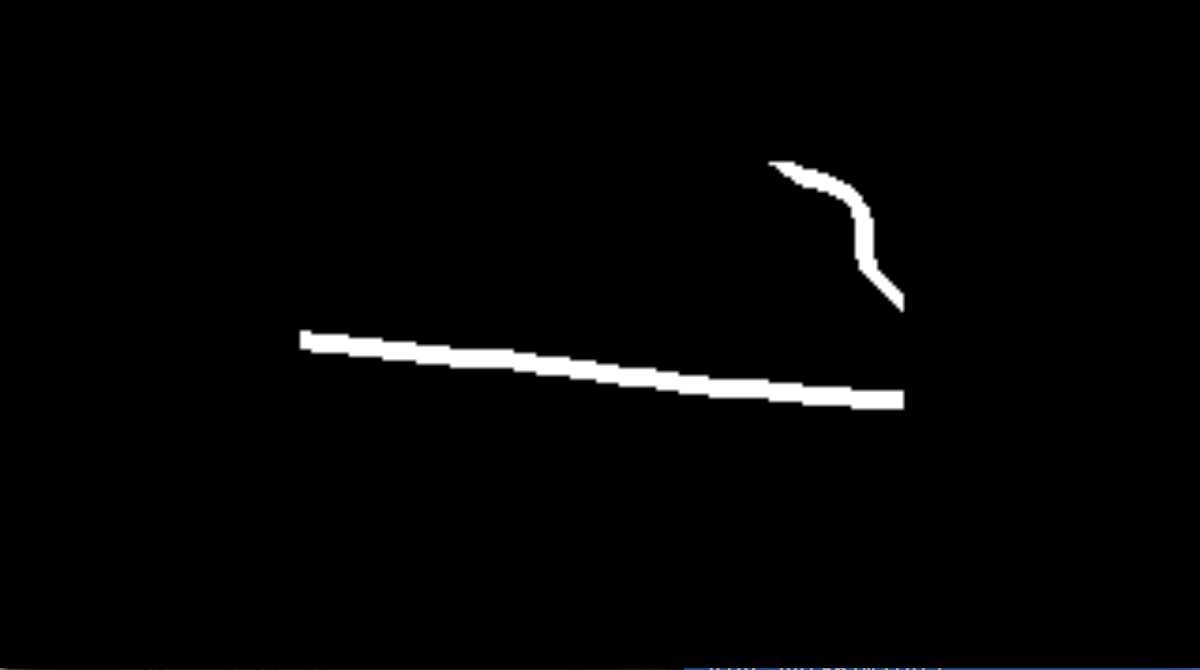
\includegraphics[width=3.1cm]{hcont.png}}%
 \subfloat[]{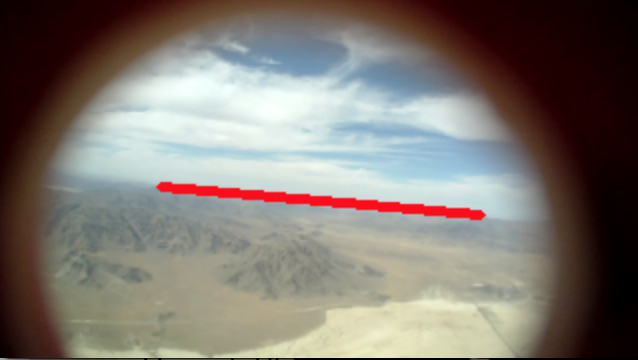
\includegraphics[width=3cm]{frame1.png}}%
 \caption{Computer vision algorithm for identifying the horizon in an image.}%
 \label{fig:cv_alg}%
\end{figure}
%%%%%%%%%%%%%%%%%%%%%%%%%%%%%%%%%%%%%%%%%%%%%%%%%%%%%%%%%

\subsection{A General Approach to Retrieving Pose from Images}
\label{sec:image_posest}

The problem of estimating the rocket's attitude from camera output is governed by the underlying projective geometry of the camera-world system. Consider the elementary graphics equation relating individual points in 3D space to camera pixels,
\begin{align}
\label{eq:cam}
\mathbf{y} &= f(\mathbf{x}) \\
&= H (R | \mathbf{t}) \mathbf{x}.
\end{align}
Here, $\mathbf{y} = (x_{image}, y_{image}, 1)^T$ gives the position of the image on the camera plane, and is a function of $\mathbf{x} = (x_{object}, y_{object}, z_{object}, 1)^T$, the position of the object. $H$ is the lens distortion matrix relating points on the ideal image plane to the actual pixel output. $R$ is the rotation matrix between the camera orientation and global coordinates, and $\mathbf{t}$ is the translation vector $(x, y, z, 1)^T$ defining the position of the camera.

Eq. \ref{eq:cam} , implies a general approach to the problem of visual pose estimation. The camera pose matrix $(R | \mathbf{t})$, which is an element of $M_{4\times3}$, may be estimated by the correct identification of five spatially distinct features. This technique is known as ``direct linear transformation". That approach, which is akin to triangulation, is subject to the same sensitivity problem as conventional 2D triangulation: the features must be separated by a large angular distance in order to properly identify the camera pose within reasonable error. The addition of more point pairs increases the certainty of the estimation.

The problem of extracting the pose of a camera from a single view is common in the computer vision and robotics literature, and the general approach described above has been efficiently implemented in the limiting case of structure-from-motion as ``visual odometry" and ``visual simultaneous localization and mapping". These approaches are very clever, but we implemented a simpler scheme to recover only pitch and yaw instead of the full pose.

By inspection of Figure \ref{fig:axes}, it can be seen that the slope and height of the horizon in a camera image represent respectively the pitch and yaw of the rocket. If the rocket pitches into the page, then the horizon will slope clockwise in the starboard camera image, and if the rocket yaws to the left, then the horizon will rise in the page; the opposite is true for the port camera. 

We make the simplification that the lens distortion matrix $H$ can be neglected, which is reasonable given that the fisheye lens results in only minimal distortion of lines passing near the center of the image (Fig. \ref{fig:horizon_overview}. Thus, in theory, raw camera output can be converted to rocket pitch and yaw measurements by identifying the slope and height of the horizon in the image, inferring the corresponding camera attitude, and correcting for the relative rotation between the camera and rocket. The specifics of this technique are detailed in Section \ref{sec:pitchyawmeas}

\begin{thebibliography}{9}
\bibitem{introtoiner} 
“Using Inertial Sensors for Position and Orientation Estimation - Now Foundations and Trends books.” [Online]. Available: https://ieeexplore.ieee.org/document/8187588. [Accessed: 03-Dec-2019].

\bibitem{appliedkalman}
R. Grover. Brown and P. Y. C. Hwang, Introduction to random signals and applied Kalman filtering: with MATLAB exercises and solutions, 3rd ed. New York: Wiley, 1997.

\bibitem{thrun}
S. Thrun, W. Burgard, and D. Fox, Probabilistic robotics. Cambridge, Mass.: MIT, 2005.

\end{thebibliography}

\end{document}
